\section{Enable remote keyboard}\label{sec:remote_keyboard}
\begin{enumerate}
    \item 0.First open remote keyboard.
\item 1.(Go to phone settings and enable remote keyboard as keyboard)
\item 2.Then go to app remote keyboard and also there, enable remote keyboard as keyboard.
\item 3.Then on pc>control panel ctrl+F "turn windows features" on or of 
\item 4.Enable Telnet Client my marking the checkbox as shown in \cref{fig:remote_keyboard}.
\begin{figure}[H]
    \centering
    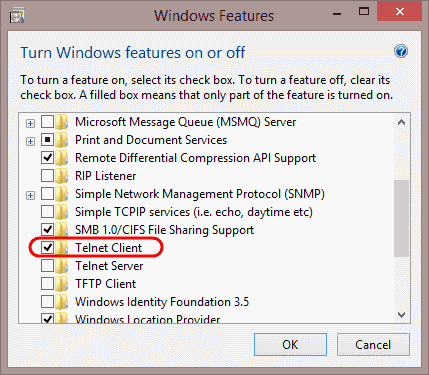
\includegraphics{images/remoteKeyboard.png}
    \caption{How to enable telnet on Windows 10}
    \label{fig:remote_keyboard}
\end{figure}
\item 5. Then start cmd and enter:
\begin{verbatim}
 telnet <ip from remote keyboard app> <port>
(including the space)
\end{verbatim}
\item 7. Then from attached calendars.ods 
    \begin{enumerate}
        \item 7.1 (When you manually add a calender by copying the google id as described here Make            sure the space after the calender id/email is gone!! so that the "/events" is also                        included.)
        \item 7.2 Use that to quickly copy calendars.ods column D into DAVdroid, (Copy column D, then paste it in the phone by rmb on cmd screen)
    \end{enumerate}
    \item 8. Open davdroid
\end{enumerate}





\section{Auto Sync all google calendars through davdroid}\label{sec:ch10}
\begin{enumerate}
    \item In public github download the PublicCodeLibrary/VBA/Google Davdroid calendar app sync/ folder. Or in excel/Google Davdroid Calendar App Sync/.
    \item Open the Excel named "calendars from gmail to davdroid V14.xlsm". That downloads google calendar website, and controls your phone.
    \item open \url{https://calendar.google.com/calendar/r/week?pli=1}
    \item Save that website as: "google.txt" in the subfolder "WebsiteSource" which is located in the same folder as the excel.
    \item install remote keyboard on phone as explained in \cref{sec:remote_keyboard} and make sure you can control phone from cmd with command: 
\begin{verbatim}
 telnet <ip from remote keyboard app> <port>
(including the space)
\end{verbatim}
    \item For me:

    \item Download opensource ahk from: \url{https://www.autohotkey.com/download/}
    \item Put the cmd with the remote keyboard connection in the right half of your screen.
    \item put the excel in the left hand side of your screen.
    \item Open davdroid on your phone, (such that the plus symbol is clickable, though do not click it.)
    \item Press the "0. get cal codes" 
    \item press the cmd with remote keyboard logged in in it, then immediately afterwards press "1. Copy Data to Phone".
\end{enumerate}

\subsection{Deleting all calendars out of Davdroid at once:}
There are at least two ways to do this:
\begin{enumerate}
    \item \textbf{Do every time:} Run the APK resetDavdroid.
    \item Do once: (Download, install and ) run app: "resetDavdroid".
    \begin{enumerate}
        \item On your external SD card create a folder named: "DAVdroidInstal" and copy the davdroid installation APK. You can get it by going to: \url{https://f-droid.org/en/packages/at.bitfire.davdroid/} and clicking: "Download APK". (currently that leads to: \url{https://f-droid.org/repo/at.bitfire.davdroid_254.apk}.
        \item rename the downloaded apk installation file to: at.bitfire.davdroid.apk
        \item Determine the location of your SD-card in your phone, in my phone it was /storage/17EE-2356. substitute the location of your SD card into the .xml code in \cref{subsubsec:taskResetDavdroid}:
        \item Copy Then copy the text of \cref{subsubsec:taskResetDavdroid} into a notepad file called resetDavdroid.txt and rename the file into resetDavdroid.xml.
        \item Import the .xml in tasker.
        \item Pick an icon for the task
        \item Export the task to an apk and install the apk:
        \begin{itemize}
            \item long press the task then three dots in top right 
            \item Package: name it to for example a.b.com
            \item Advanced Configuration: Check the box
            \item At Extra permissions enter:
\begin{verbatim}
android.permission.WRITE_SECURE_SETTINGS
\end{verbatim}
            \item That exports the app to: (Internal) storage card/media/tasker/factory/kids/ 
 .apk which in my case had the exact path name:
\begin{verbatim}
/storage/emulated/0/Tasker/factory/kids/
\end{verbatim}       
        \end{itemize}
        \item ..Then run the app to reset Davdroid. That clears out all calendars. 
            \begin{enumerate}
                \item When it prompts for root access, mark "do not ask again" and press OK.
                \item When then applock asks to lock (the freshly installed) Davdroid click Cancel/NO.
                \item (Actually export/build and install- the app by pressing the back button on the top left of the screen).
            \end{enumerate}
    \end{enumerate}
\end{enumerate}
\subsubsection{.xml code reset Davdroid task}\label{subsubsec:taskResetDavdroid}
\begin{verbatim}
<TaskerData sr="" dvi="1" tv="5.2.bf1">
    <Task sr="task28">
        <cdate>1546182301418</cdate>
        <edate>1546204083437</edate>
        <id>28</id>
        <nme>ResetDAVdroid</nme>
        <pri>100</pri>
        <Kid sr="Kid">
            <eperm0>android.permission. WRITE_SECURE_SETTINGS</eperm0>
            <launchID>28</launchID>
            <pkg>a.b.com</pkg>
            <vnme>1.0</vnme>
            <vnum>4</vnum>
        </Kid>
        <Action sr="act0" ve="7">
            <code>123</code>
            <Str sr="arg0" ve="3">pm uninstall at.bitfire.davdroid</Str>
            <Int sr="arg1" val="0"/>
            <Int sr="arg2" val="1"/>
            <Str sr="arg3" ve="3"/>
            <Str sr="arg4" ve="3"/>
            <Str sr="arg5" ve="3"/>
        </Action>
        <Action sr="act1" ve="7">
            <code>123</code>
            <Str sr="arg0" ve="3">pm install /storage/17EE-2356/DAVdroidInstal/at.bitfire.davdroid.apk</Str>
            <Int sr="arg1" val="0"/>
            <Int sr="arg2" val="1"/>
            <Str sr="arg3" ve="3"/>
            <Str sr="arg4" ve="3"/>
            <Str sr="arg5" ve="3"/>
        </Action>
        <Img sr="icn" ve="2">
            <nme>hd_content_discard</nme>
        </Img>
    </Task>
</TaskerData>
\end{verbatim}
For me the location is: %mega8/mob/18-12-30 custom Apps/

\subsection{TODO:}
\begin{enumerate}
    \item Get calendars through api
    \item correct long names of imported .cal files from mytimetable
    \item automate adapting loop of .ahk to nr of calendars.
    \item stop doing beun de haas and just do it all inside the smartphone.
    \item check if opentasks has a better calendar synchronization than taskwarrior andorid task apk.
\end{enumerate}
\subsection{Try to write the calendars directly into the phone storage for Davdroid}
Davdroid does not store any calendars, those are stored in their normal place in the android operating system. However, it uses a file services.db to change those files is what I understood. The changing happens using sql. The following things are unclear:
\begin{itemize}
    \item It is unclear wether the davdroid settings are stored in the services.db or whether the services.db is just a sort of api/handler that accesses the calendar settings of davdroid somehow.
    \item Are there a lot of extra settings changed within Davdroid when you add a calendar the conventtional way. E.g. If I happen to find the location where the calendar settings of Davdroid are stored, and I would be able to perfectly replicate add a calendar there (by for example, first adding one just using davdroid correctly, copying the file content that contains that specific calendar setting, and deleting and re-installing davdroid (including data) and restoring that specific calendar file content in that calendar-settings-file.) Or are there separate processeses like for example encryption keys uniquely created if you verify for example the base url in the normal davdroid way, which I did not do by simply pasting in the calendar settings?
    \item Where are the actual settings stored, derive that from the answers given by rc2822.
    \item How to decrypt/encrypt/store the passwords for the gmail acocunt?
\end{itemize}
 So presumably, you want to find the services.db to see how you can inject your calendar settings into davdroid.
Source: \url{https://forums.bitfire.at/topic/1834/location-of-calendar-settings-storage-on-lineageos-14-1-with-davdroid-1-11-4-1-ose/6}
Services.db is not found, however, a similar calendars.db is found at location:
\begin{verbatim}
/data/data/com.android.providers.calendar/databases/calendar.db
\end{verbatim}
This contains at least the list of calendars of android itself, it is not yet sure if it also contrains the synchronisation settings of davdroid.



\begin{enumerate}
    \item The services.db is located in the root as: /data/data/at.bitfire.davdroid/databases/services.db
    \item To read the services.db file look at: \url{https://developer.android.com/studio/command-line/adb#othershellcommands}
    \item with adb and the following commands you can manipulate the database file:
\begin{verbatim}
adb -s emulator-5554 shell
sqlite3 /data/data/com.example.app/databases/rssitems.db
SQLite version 3.3.12
Enter ".help" for instructions
\end{verbatim}    
\item 

https://www.sqlite.org/download.html

\item Found the services.db file relative to the root of my devices as: /data/data/at.bitfire.davdroid/databases/services.db
\item Exported and visually inspect the database with SQlite studio to determine which tables the services.db contain.
\item That allows for conversion of the services.db to a .csv file according to: \url{http://www.sqlitetutorial.net/sqlite-tutorial/sqlite-export-csv/.}
\item That allows for reverse engineering the database, to generate new ones with custom calendars.
\item The next step however, is to determine where and how the password is stored by Davdroid, for for example the accompanying google accounts for base-url added google calendars.
\item the password is stored (in plain text in 2016) in androids default location using the android account manager: \url{https://developer.android.com/reference/android/accounts/AccountManager#setPassword%28android.accounts.Account,%20java.lang.String%29} and \url{https://developer.android.com/reference/android/accounts/AccountManager#getPassword(android.accounts.Account)}. That could mean you should use an api to get the password. 
\item According to \url{https://forums.bitfire.at/topic/264/view-changes-properties-of-an-existing-davdroid-account/21} the passwords are stored in /data/system/users/0/accounts.db. I have not yet been able to find that database but I will look into it in more detail.
\end{enumerate}
\noindent Using 